\documentclass[]{article}
\usepackage{lmodern}
\usepackage{amssymb,amsmath}
\usepackage{ifxetex,ifluatex}
\usepackage{fixltx2e} % provides \textsubscript
\ifnum 0\ifxetex 1\fi\ifluatex 1\fi=0 % if pdftex
  \usepackage[T1]{fontenc}
  \usepackage[utf8]{inputenc}
\else % if luatex or xelatex
  \ifxetex
    \usepackage{mathspec}
  \else
    \usepackage{fontspec}
  \fi
  \defaultfontfeatures{Ligatures=TeX,Scale=MatchLowercase}
\fi
% use upquote if available, for straight quotes in verbatim environments
\IfFileExists{upquote.sty}{\usepackage{upquote}}{}
% use microtype if available
\IfFileExists{microtype.sty}{%
\usepackage{microtype}
\UseMicrotypeSet[protrusion]{basicmath} % disable protrusion for tt fonts
}{}
\usepackage[margin=1in]{geometry}
\usepackage{hyperref}
\hypersetup{unicode=true,
            pdftitle={Characterisation of model species interactome available from primary molecular interaction databases},
            pdfauthor={Vitalii Kleshchevnikov},
            pdfborder={0 0 0},
            breaklinks=true}
\urlstyle{same}  % don't use monospace font for urls
\usepackage{graphicx,grffile}
\makeatletter
\def\maxwidth{\ifdim\Gin@nat@width>\linewidth\linewidth\else\Gin@nat@width\fi}
\def\maxheight{\ifdim\Gin@nat@height>\textheight\textheight\else\Gin@nat@height\fi}
\makeatother
% Scale images if necessary, so that they will not overflow the page
% margins by default, and it is still possible to overwrite the defaults
% using explicit options in \includegraphics[width, height, ...]{}
\setkeys{Gin}{width=\maxwidth,height=\maxheight,keepaspectratio}
\IfFileExists{parskip.sty}{%
\usepackage{parskip}
}{% else
\setlength{\parindent}{0pt}
\setlength{\parskip}{6pt plus 2pt minus 1pt}
}
\setlength{\emergencystretch}{3em}  % prevent overfull lines
\providecommand{\tightlist}{%
  \setlength{\itemsep}{0pt}\setlength{\parskip}{0pt}}
\setcounter{secnumdepth}{0}
% Redefines (sub)paragraphs to behave more like sections
\ifx\paragraph\undefined\else
\let\oldparagraph\paragraph
\renewcommand{\paragraph}[1]{\oldparagraph{#1}\mbox{}}
\fi
\ifx\subparagraph\undefined\else
\let\oldsubparagraph\subparagraph
\renewcommand{\subparagraph}[1]{\oldsubparagraph{#1}\mbox{}}
\fi

%%% Use protect on footnotes to avoid problems with footnotes in titles
\let\rmarkdownfootnote\footnote%
\def\footnote{\protect\rmarkdownfootnote}

%%% Change title format to be more compact
\usepackage{titling}

% Create subtitle command for use in maketitle
\newcommand{\subtitle}[1]{
  \posttitle{
    \begin{center}\large#1\end{center}
    }
}

\setlength{\droptitle}{-2em}
  \title{Characterisation of model species interactome available from primary
molecular interaction databases}
  \pretitle{\vspace{\droptitle}\centering\huge}
  \posttitle{\par}
  \author{Vitalii Kleshchevnikov}
  \preauthor{\centering\large\emph}
  \postauthor{\par}
  \predate{\centering\large\emph}
  \postdate{\par}
  \date{21 December 2016}


\begin{document}
\maketitle

{
\setcounter{tocdepth}{2}
\tableofcontents
}
The report was published on 2017-04-27. All data used in the report as
available on 2017-04-24.

\section{Outline}\label{outline}

\begin{enumerate}
\def\labelenumi{\arabic{enumi}.}
\tightlist
\item
  Abstract
\item
  Introduction
\item
  Methods
\item
  Results and discussion

  \begin{itemize}
  \tightlist
  \item
    how available interactome covers the proteome
  \item
    IMEx(IntAct) vs Biogrid
  \item
    which proteins are missing
  \item
    interaction detection biases
  \item
    study bias: the more articles, the more interactions
  \item
    which proteins are IMEx(IntAct), Biogrid and high-throughput
    datasets enriched in?
  \end{itemize}
\item
  Conclusion
\end{enumerate}

\section{Abstract}\label{abstract}

\section{Introduction}\label{introduction}

The structure and the function of the cell arise from interactions
between molecules inside and outside it. Though proteins, nucleic acids,
lipids and small molecules can all form important interactions, studies
and literature focus mainly on interactions between proteins and other
macromolecules. We can discover and study these molecular interactions
using a number of experimental and computational techniques. This study
focuses on molecular interactions identified in the experimental
setting, most of which are represented in the literature and databases
by protein-protein interactions (also protein-DNA interactions obtained,
for example, by ChIP-Seq, but those are traditionally incorporated into
genomic databases).

Based on the information detection methods can provide towards ground
truth we can classify interactions in three types: binary interactions
and associations. Binary interactions are the interactions between two
components, for example, two specific proteins, some detection methods
(e.g.~two-hybrid) identify those. To understand associations, we need to
imagine we know proteins A, B and C constitute a complex and interact as
shown in a figure 1 A. When we conduct an experiment, we choose the bait
(the molecule experimentally treated to capture its interacting partners
- called preys) to be protein A, and by detection method
(e.g.~affinity-purification mass spectrometry) we get both protein B and
protein C detected as preys. Next step is to translate bait-prey
relationship into a model of reality like the one shown in the figure 1
A. We call interactions between A-B and A-C associations because we
cannot infer the true relationship between A, B, and C from this
experiment design. In the other words, establishing that proteins are in
direct physical contact is really challenging. However, to represent
associations in a tabular format with each row corresponding to one
interaction (e.g.~A-B) we need to expand those. Two ways are commonly
used to expand interactions, hub and spoke expansion, both shown in the
figure 1 B.

\paragraph{Defining interactome}\label{defining-interactome}

The aggregation of all components and their interactions into a single
network result in what we call interactome, the whole of all molecular
interactions. You can also look into the subset of this network, for
example, you can select only proteins, only those proteins that are
expressed in the brain, and only the interactions between this protein
identified experimentally in the brain cells. This example reflects the
complexity and the diversity of the interactome - which is what you
would expect from a system underlying the complexity and the diversity
of the cell types, cellular behaviours, and functions. For the same
reason, only by studying these interactions and how they change in
specific cell types and under specific circumstances in combination with
the functional analysis we can decipher cellular regulatory networks.
The ultimate goal of the research in the field would be to capture all
physical interactions and thoroughly describe them while avoiding false
discoveries.

\paragraph{Experimental approaches for discovering
interactions}\label{experimental-approaches-for-discovering-interactions}

Experimental protein interaction detection methods can be classified
into 3 main categories based on the evidence they provide and whether
they can be used in a high-throughput manner: The first category is
formed by methods using affinity purification of the bait and all the
prey associated with it. Following that, preys can be identified using
western-blotting and specific antibodies or using mass-spectrometry,
which can be done in a high-throughput manner {[}Mann, {]}. The main
advantage of these methods is the ability to quantitatively characterise
interactions {[}Mann, {]} and capture many prey proteins per bait - the
latter, however, presents the disadvantage of dealing with associations.
The main disadvantage of these techniques is that for the reliable
result it requires all interacting proteins to be soluble {[}{]}. The
second category is formed by protein complementation techniques which
include two-hybrid (transcription factor complementation), the most
widely used interaction detection method (including high-throughput
experiments). In this method, pairs of proteins are tested for
interaction and therefore all discovered interactions are binary (the
main advantage of this method). Classic implementation of two-hybrid
requires proteins to be soluble as well {[}{]}, however, two-hybrid for
membrane proteins was also developed {[}{]}. The main disadvantage of
two-hybrid methods are that they allow only qualitative characterisation
of interactions {[}{]}, are usually performed in yeast (thus, have a
lower sensitivity) and are highly prone to false-positive results
{[}{]}. Final category consists of methods based on the structure of the
protein complex. They can provide valuable information on how exactly
physical interaction occurs but as for now are extremely labor-intensive
and will always need complementary experiments showing if the proteins
actually interact in the cellular context.

\paragraph{Challenges of
interactomics}\label{challenges-of-interactomics}

Four big challenges substantially complicate the study of molecular
interactions, especially on the whole organism scale. The first being
that we don't know the true nature of underlying our experimental
results (all assays provide evidence that interaction is possible and
some can provide quantitative description, but all are prone to error
and the problem described in the figure 1 A) which lead to the necessity
of combining interaction data from multiple experiments and complex
statistical evaluation of how probable the interaction is based on that
data (Bayesian approach {[}1{]}) rather than receiving confident
yes-or-no result from single experiment. Interaction databases make an
effort to score the interactions based on supporting evidence, however,
this is usually done with non-probabilistic heuristic approaches, like
MI score {[}PMCID: PMC4316181{]}.

The second big challenge is the problem of ``noise'' - or false
positives. Different interaction detection experiments are prone to
these errors for different reasons, for example, in-vitro experiments
(e.g.~TAP-MS) may allow the interaction between proteins which are
normally included in separate cellular compartments. Specific groups of
proteins (based on their physical or chemical properties) may have a
higher susceptibility to false positives, for example, intermediate
filaments (e.g.~nuclear lamins) have low solubility under non-denaturing
conditions necessary for affinity-purification based techniques, which
may lead to artifactual results. However plausible, this particular
problem lacks empirical evidence and requires more investigation. A more
general problem of noise will be addressed by more proteome-scale
interactomics experiments (which can include enough samples to guarantee
low false positive rate while still identifying interactions).

The third big challenge is that our knowledge of interactome is
incomplete and arises from the fact that experimental approaches have
low statistical power and often miss out some real interactions. Also,
many proteins, especially for non-popular model species, were not
researched for protein interactions.

The final challenge contributes to the ``incomplete interactome''
problem but is grounded in the fact that not all protein interaction
discovered and published are included in protein interaction databases.
In the other words, this is database curation problem. More than 100
public databases containing protein interactions are available now.
These databases differ: - by the types of data they include
(e.g.~computational prediction, manual curation from experimental
articles - primary, aggregated data from many primary databases -
secondary),\\
- the level of detail captured from articles to describe interactions,\\
- how often and if they are updated with new data.\\
The level of detail ranges from only mentioning the pairs of interactors
and heuristic score assigned to them (STRING, updated once in 2 years)
to the ones containing experiment details (detection method, bait/prey
status, if available - quantitative data, experiment setup, protein
variants), such as IntAct {[}PMCID: PMC3703241{]}. The amount of
interaction data generated per year is growing exponentially making
manual curation of all this data into primary databases a daunting task.
To prioritise curation efforts and reduce redundancy between databases
(to curate different data using the same standards) IMEx consortium was
formed in 2012 {[}PMCID: PMC3703241{]}. IMEx-compliant databases include
all big primary databases excluding only BioGRID (which curates at the
lower level of detail) and not active legacy databases.

\paragraph{Motivation for this study}\label{motivation-for-this-study}

Solving some of these challenges may be easier than the others. In
particular, to solve the last challenge we can prioritise curation
efforts for already published interactions to cover unrepresented
proteins and we can encourage authors to submit their results to the
databases prior to publishing. We can also encourage research of
underrepresented parts of the interactome. However, for both of those
aims, we need to characterise the interactome already present in
interaction databases. Specifically, to learn how available interactome
covers the proteome of main model species, if there are any biases to
proteins with no available interactions and if any major protein
interaction detection methods exhibit any biases towards specific groups
of proteins. The other helpful to look at the problem is to search for
underrepresented in interaction databases but in general well-researched
proteins.

\section{Aims of the study}\label{aims-of-the-study}

\begin{enumerate}
\def\labelenumi{\arabic{enumi}.}
\item
  Find out how available interactome covers the proteome of main model
  species. Considering either all UniProtKB or SwissProt entries only as
  the proteome (canonical identifiers as well as protein isoforms).
  Consider all interactions from IMEx-compliant databases as
  interactome.
\item
  Compare the coverage of proteome by interactome from IMEx to the
  interactome from BioGRID (the other major primary database).
\item
  Find out if proteins with no available interactions stand out by
  specific functions (Gene Ontology, GO: biological process and
  molecular function), cellular localisation (GO), molecular mass, or
  protein evidence status from SwissProt
\item
  Find out if major protein interaction detection methods (two-hybrid
  and AP-MS, AP-WB?) exhibit any bias towards biochemical properties of
  the proteins involved (mass, disordered regions, hydropathy, the
  fraction of charged residues)
\item
  What is the relationship between the number of interactions or MI
  score and the number of publications or GO terms per protein?
\item
  Are proteins with a higher fraction of intrinsically disordered
  domains more likely to have interactions available and do they have
  more interactions (if normalised for how well-studied proteins are)?
\item
  Find out if there are any proteins which are in general well
  researched (many associated publications or manual GO annotations) but
  underrepresented in IntAct (low MI score)
\item
  If that is possible to measure: do intermediate filaments (or other
  highly insoluble proteins) really have higher rates of
  false-discovered interactions?
\end{enumerate}

\section{Methods - data processing and
analysis}\label{methods---data-processing-and-analysis}

\subsubsection{Getting proteome from
UniProtKB}\label{getting-proteome-from-uniprotkb}

Whole proteome (all UniProtKB) for each species was downloaded
programmatically in R using UniProt rest API. SwissProt-proteome was
subset from the whole proteome by reviewed status column. UniProt
identifies proteins by UniProtKB/AC (e.g.~P04637, accession) which does
not distinguish between protein isoforms. UniProt aggregates isoform
information and identifiers (e.g.~P04637-4) in a separate column with
zero to many isoforms per each UniProtKB accession. To generate proteome
list which includes protein isoforms, isoform accessions were extracted
and combined with the list of generic accessions. In this analysis,
protein evidence status and protein mass are only attributed to generic
accessions.

\subsubsection{Getting and transforming interactome data from IMEx
databases and
BioGRID}\label{getting-and-transforming-interactome-data-from-imex-databases-and-biogrid}

Interactome from all IMEx databases was downloaded programmatically in R
using PSIQUIC package from Bioconductor {[}Paul Shannon (2015).
PSICQUIC{]}. IMEx databases include IntAct, MINT, bhf-ucl, MPIDB,
MatrixDB, HPIDb, I2D-IMEx, InnateDB-IMEx, MolCon, UniProt, MBInfo. The
list of interactions (pairs of interactors) was transformed into the
list of interactors preserving interactor identifiers, the type of
interactor identifier, species information and the database interaction
originates from. Only unique proteins wereIMEx databases contain
interactions between proteins, RNA, DNA and small molecules, moreover,
these interaction may involve molecules originating from different
species. Therefore, to perform by species interactome/proteome
comparison there is a need to remove non-UniProtKB/AC molecule
identifiers (which removes non-protein molecules, although, may also
remove a small fraction of proteins which have no UniProtKB/AC) and
there is a need to remove proteins originating from other species. Also,
entries in IMEx databases has to be cleaned of tags and textual
descriptions (``taxid:9606(human-h1299)\textbar{}taxid:9606(Homo sapiens
lung lymph node carcinoma)'' to ``9606'') to make further analysis
easier and cleaner. Next, when provided in the research articles protein
isoform information is always included in IMEx databases, so to perform
analysis excluding isoform information UniProtKB/AC were cleaned of -N
suffix (P04637-4 to P04637).

\subsubsection{Disordered regions and physical
properties}\label{disordered-regions-and-physical-properties}

Information on disordered region content and biochemical properties of
individual proteins were obtained from the dataset generated by Vincent
and Schnell in 2015 {[}{]}. Briefly, Vincent and Schnell used a number
of disorder prediction algorithms (IUPred and DisEMBL) and their
consensus to generate disordered region predictions for each protein
which was be used to calculate the fraction of disordered regions in a
protein. In addition, Vincent and Schnell used localCIDER version 0.1.7
(Classification of Intrinsically Disordered Ensemble Regions) to
calculate physical properties such as a fraction of charged residues,
mean hydrophobicity or charge separation for each protein. This was done
for 10 eukaryotic proteomes and written to SQLite-database which was
made available online.

\subsubsection{Gene ontology enrichment
analysis}\label{gene-ontology-enrichment-analysis}

coming soon

\section{Results}\label{results}

\subsection{1. How well available interactome covers the
proteome}\label{how-well-available-interactome-covers-the-proteome}

\subsubsection{Available interactome covers substantial fraction of the
reviewed proteome of main model
species}\label{available-interactome-covers-substantial-fraction-of-the-reviewed-proteome-of-main-model-species}

In this section, we compare the list of all proteins (per species) in
Uniprot (reviewed part (or SwissProt) - Figure 2, reviewed and
unreviewed parts (or all UniProtKB: SwissProt + trEMBL) - Supplementary
Figure 1) to the list of proteins which have interaction partners
annotated in IMEx consortium databases. Non-canonical protein isoform
identifiers (P32054-1) were converted to canonical identifiers (P32054)
resulting in interactions ``any isoform to any isoform'' (Venn diagrams
on the right) or isoform identifiers were preserved (Venn diagrams on
the left). You can see that adding isoform information adds more
proteins to the SwissProt list but not so many proteins to the IMEx
list.

\begin{figure}[htbp]
\centering
\includegraphics{final_report_files/figure-latex/IMEx_vs_Uniprot_venndiagram-1.pdf}
\caption{Figure 2}
\end{figure}

Overall - the best interactome annotated by IMEx databases is baker's
yeast, 2nd best interactome is \emph{E.coli}. All other interactomes
cover less than the half of their respective proteome (all UniProtKB,
Supplementary figure 1). The overlap between the interactome and
reviewed proteome (SwissProt) is significantly better. A large fraction
of human, mouse, arabidopsis proteins-interactors and more than a half
of drosophila and \emph{C.elegans} proteins-interactors are absent in
SwissProt (but included in trEMBL) -- suggesting under-annotation by the
SwissProt-Uniprot team. Protein isoforms (in multicellular model
organisms) are almost not annotated in the interactome. Human is an
exception -- 2656 protein isoforms out of 22049. Other molecular
interaction databases (active BioGRID, inactive HPRD) do not record
isoform information.

\subsection{2. BioGRID database (as obtained from Mentha) overlaps
significantly with IMEx
databases}\label{biogrid-database-as-obtained-from-mentha-overlaps-significantly-with-imex-databases}

BioGRID database is the second major primary protein interaction
database which when combined with IntAct contains all interactions
information which has been curated to currently active public databases
(major inactive or legacy databases include HPRD and BIND). BioGRID is
characterised by shallow curation level (retains only some information
about the interaction and the experiment) and identifies proteins using
Entrez Gene ID while IntAct uses UniProtKB identifiers. Entrez Gene ID
does not allow to distinguish between different protein isoforms. In our
analysis, this difference introduces additional mapping step (Gene ID to
UniProtKB). Mentha database has imported all BioGRID-stored interactions
and has mapped Gene ID to UniProtKB, so we used Mentha to get
BioGRID-stored interactions. Mentha doesn't import interactions for
\emph{E.coli}, therefore \emph{E.coli} is absent in this analysis.
BioGRID has recently incorporated a large-scale study aimed, in part,
for find interacting partners for the proteins missing them {[}{]}.

\begin{figure}[htbp]
\centering
\includegraphics{final_report_files/figure-latex/biogrid_vs_IMEx_vs_Uniprot_venndiagram-1.pdf}
\caption{Figure 4}
\end{figure}

Overall, BioGRID overlaps with IMEx to a large extent. Nonetheless, for
all of the species we have looked at, BioGRID has annotated some
proteins (and their interactions) which are not annotated in IMEx.
BioGRID stores substantially more interactions for arabidopsis and quite
a lot of human and mouse interactions.

\subsection{3. Mouse and human proteins are commonly combined for
interaction
experiments}\label{mouse-and-human-proteins-are-commonly-combined-for-interaction-experiments}

The fact that researchers tend to put proteins from other species
(mostly human) into mouse experiments or tend to put mouse proteins into
cells from other species (mostly human) is also common for interaction
detection experiments and is clearly seen in figure 3: half of the mouse
interactors are from the other species. This holds true both for IMEx
databases (figure 3) and for BioGRID. However, this analysis doesn't
show which proteins (mouse or human) were used as bait to capture
interactions in which cells (mouse or human).

Figure 3 also displays how many interactors do not have Uniprot
identifiers - those are small molecules, RNA, DNA or a small fraction of
proteins not mapped to UniProt. Big fraction of \emph{C.elegans}
interactors are coming from single experiment mapping transcription
factors to their sites {[}{]}

\begin{figure}[htbp]
\centering
\includegraphics{final_report_files/figure-latex/IMEx_vs_Uniprot_N_Uniprot_Species-1.pdf}
\caption{Figure 3}
\end{figure}

Interchangeable use of mouse and human proteins generates interaction
data which is hard to reuse and introduces imprecision due to the fact
that it requires the mapping between homologous proteins. However, this
may not be the biggest problem with studying the interactions between
mouse and human proteins and trying to correctly interpret results.
Recent studies of intrinsically disordered proteins show that linear
amino acid motifs located in disordered regions frequently mediate
protein-protein interactions {[}{]}, for example, the disordered region
of p53 mediates its ability to recruit transcription-activating proteins
to the promoter {[}{]}. More importantly, these linear amino acid motifs
can evolve quickly, for example, allowing cancer cells to escape control
by P53 {[}{]}. So, while the interaction between mouse protein A and
human protein B can exist, that might not be true for the interaction
between human protein A and human protein B, and vice-verse. On the
other hand, some researchers advocate that interactions important for
the cellular function should be conserved between species {[}{]}.

Surprisingly, 19438 interactions between mouse and human proteins were
discovered in human rather than mouse cells (only 1233) suggesting that
researchers use mouse rather than human proteins as baits (1158 mouse
baits total, 5606 human preys total, including isoforms, from 441
publications) to find interactions directly relevant to human
interactome research, including human disease.

\subsection{4. Which proteins are missing interaction
evidence?}\label{which-proteins-are-missing-interaction-evidence}

Characterising the properties of proteins missing interaction evidence
can help prioritise curation efforts. By looking for proteins missing
interaction evidence and involved in particular biological function (as
described by Gene Ontology) or particular disease we can complete
missing part of the interactome.

\subsubsection{Olfactory receptors are a major group of human proteins
not represented in
IntAct}\label{olfactory-receptors-are-a-major-group-of-human-proteins-not-represented-in-intact}

coming soon

\includegraphics{final_report_files/figure-latex/human_not_in_IMEx_protein_properties_GOenrichment-1.pdf}
\includegraphics{final_report_files/figure-latex/human_not_in_IMEx_protein_properties_GOenrichment-2.pdf}

\includegraphics{final_report_files/figure-latex/human_not_in_IMEx_protein_properties_GOdepleted-1.pdf}

\includegraphics{final_report_files/figure-latex/GO_enrichment_map-1.pdf}
\includegraphics{final_report_files/figure-latex/GO_enrichment_map-2.pdf}

\subsubsection{Human proteins with no available interactions (from IMEx)
are on average shorter than the proteins with interactions
available}\label{human-proteins-with-no-available-interactions-from-imex-are-on-average-shorter-than-the-proteins-with-interactions-available}

Protein length or mass are physical properties of a protein which can,
in theory, influence it's usage as a bait in experiments and it's
detection in case methods depend on protein length. Proteins length is
also important biologically. Longer proteins can have multiple
functional domains and, therefore, more interactions. The distribution
of protein mass has a very long right tail - there are much more big
proteins than a normal distribution would predict (Supplementary figure
3), which only allows using non-parametric statistical tests (Wilcox
test). Log10 transformation of protein mass, though, makes extreme
values less extreme and is approximately normally distributed.

\begin{figure}[htbp]
\centering
\includegraphics{final_report_files/figure-latex/human_not_in_IMEx_proteins_are_shorter_density-1.pdf}
\caption{Figure 5}
\end{figure}

This difference in protein mass between proteins present and absent in
the interactome is highly unlikely to occur by chance (Wilcox rank test
(Mass, Da, 95\% confidence interval: -1.3\times 10\^{}\{4\},
-1.11\times 10\^{}\{4\}, p-value: 6.76\times 10\^{}\{-142\}) and Student
t-test(log10 of Mass, Da, 95\% confidence interval: -0.153, -0.132,
p-value: 4.68\times 10\^{}\{-143\}) on the whole population of proteins,
Monte-Carlo sampling (is it useful?), permutation of labels followed by
Wilcox rank test (is it useful?) - Supplementary figure 3,4,5). Removing
416 olfactory receptors, evidently, does not change this trend (Wilcox
rank test on Mass, Da, 95\% confidence interval:
-1.28\times 10\^{}\{4\}, -1.08\times 10\^{}\{4\}, p-value:
2.98\times 10\^{}\{-121\}).

\subsubsection{Major experimental role types (bait/prey/neutral
component) are not substantially influenced by the mass of the
protein}\label{major-experimental-role-types-baitpreyneutral-component-are-not-substantially-influenced-by-the-mass-of-the-protein}

The experimental role of the protein (bait/prey/neutral component) can,
in theory, be influenced by protein mass. For example, it may be easier
to clone shorter proteins for use as bait/prey. So it important to see
if the experimental role is really influenced by protein mass.

\begin{figure}[htbp]
\centering
\includegraphics{final_report_files/figure-latex/human_not_in_IMEx_bait_vs_non_bait-1.pdf}
\caption{Figure 5}
\end{figure}

We can now select only the most frequent experimental roles

\begin{figure}[htbp]
\centering
\includegraphics{final_report_files/figure-latex/human_not_in_IMEx_bait_vs_non_bait2-1.pdf}
\caption{Figure 5}
\end{figure}

Evidently, the experimental role of a protein is not substantially
influenced by the mass of the protein.

\subsubsection{Most of the human proteins with no available interactions
(from IMEx databases) are membrane
proteins}\label{most-of-the-human-proteins-with-no-available-interactions-from-imex-databases-are-membrane-proteins}

coming soon

\subsubsection{If a protein is missing protein evidence in Uniprot it is
also more likely to be missing from IMEx
databases}\label{if-a-protein-is-missing-protein-evidence-in-uniprot-it-is-also-more-likely-to-be-missing-from-imex-databases}

coming soon

\subsection{5. Proteins missing interaction evidence are not associated
with specific
disease}\label{proteins-missing-interaction-evidence-are-not-associated-with-specific-disease}

\includegraphics{final_report_files/figure-latex/disease_enrichment_map-1.pdf}

\subsection{5. Do major protein interaction detection methods
(two-hybrid and AP-MS) exhibit a bias towards biochemical properties of
the proteins
involved?}\label{do-major-protein-interaction-detection-methods-two-hybrid-and-ap-ms-exhibit-a-bias-towards-biochemical-properties-of-the-proteins-involved}

The problem of bias in interactomics is often discussed in research
papes and in the community. Now we will focus on the bias in the
experimental detection method. We choose to compare two major families
of methods: two-hybrid and affinity-purification-mass-spectrometry
(AP-MS). We define two-hybrid using PSI-MI ontology: detection method =
``transcriptional complementation assay'' (MI:0018) - all methods which
belong to this type (which are children terms in the ontology). We
define AP-MS using two PSI-MI ontology terms: detection method =
``affinity chromatography technology'' (MI:0004) and participant
identification method = ``partial identification of protein sequence''
(MI:0433). We get interactions detected using these methods by querying
PSICQUIC. We use word formulations rather than ontology term identifiers
because PSICQUIC package in R is not equipped to handle quotes in the
query text (``MI:0004'' AND ``MI:0102'').

\subsubsection{AP-MS is biased towards longer
proteins}\label{ap-ms-is-biased-towards-longer-proteins}

Unlike the experimental role type, whether a protein interaction is
detected using a particular interaction detection method is influenced
by the mass of that protein.

\begin{figure}[htbp]
\centering
\includegraphics{final_report_files/figure-latex/interaction_types_combine_and_plot-1.pdf}
\caption{Figure 6}
\end{figure}

The statistical significance of the difference in protein mass across
protein detection methods was tested using linear model approach. Linear
model offers way to perform multiple statistical tests (ANOVA and
posthoc ttests) in R. Linear model takes a group assignment for a
protein (only two-hybrid, only AP-MS, both two-hybrid and AP-MS, other
methods - a vector 0s and 1s where 1 show which group a protein belongs
to) and the mass of that protein. Using these parameters for each of the
proteins linear model can learn the mean of each group as well as
provide a way to calculate errors for each of the between-group
comparisons. The robust linear model used for this test is less
sensitive to the extreme values. The results of statistical tests can be
visualised on a plot. In the box plot below, each vertical arrow points
to the mean mass of the proteins in a particular group. The middle line
of the boxplot represents a median which happens to coincide with mean
because the distribution of logarithm base 10 of mass is approximately
normally distributed. Each yellow arrow shows the p-value and the
difference in protein mass between two corresponding groups.

\begin{figure}[htbp]
\centering
\includegraphics{final_report_files/figure-latex/protein_length_det_method_rlm-1.pdf}
\caption{Figure 7. Does rlm require normally distributed data?}
\end{figure}

The figure X shows that the mass of the proteins which were identified
interacting using AP-MS technique is on average higher that the mass of
the proteins identified using two-hybrid or the other methods.

\subsection{6. The number of interactions (or MI score) is associated
with the number of
publications}\label{the-number-of-interactions-or-mi-score-is-associated-with-the-number-of-publications}

The problem of better-studied proteins having more interactions despite
all proteins having similar amounts of Mendelian-type mutations and
therefore similar functional significance has been discussed in the
literature a few years ago {[}{]}. So we decided to have a fresh look
and explore the problem more deeply. Interaction is defined by two
proteins which form it regardless of how many times these proteins were
spotted interacting. MI score is an empirical score proposed by IMEx
consortium to evaluate the evidence that supports each given interaction
{[}{]}. Not every interaction has enough evidence to get an MI score. We
have counted the number of interactions for each protein (Figure 8) and
summed MI scores over interactions for each protein (Figure 9, this can
be seen as the number of interactions combined with the confidence we
have for their existence). We define a large-scale study as a study
which provided more than 100 interactions in IntAct (counting by
interaction identifiers). The number of publications per gene was
counted using NCBI gene to PubMed ID conversion table.

Just to be clear: for each protein which has all interacting partners
identified exclusively by large-scale studies, or small-scale studies,
or both large-scale and small-scale studies we show the number of
interacting partners (which were indentified in those three types of
studies) and the number of publications, any type of study involving the
gene which codes for that particular protein. To emphasise, in the
figures below, we do not examine whether the same protein has a
different number of interacting partners coming from large-scale or
small-scale studies, we aggregate all those proteins into one group and
count the total number of interacting partners each protein has (each
particular interaction may have been identified in many large-scale
studies, or many small-scale studies, or both large-scale and
small-scale studies).

The figures below show the number of interacting partners associated
with the number of publications (x-axis) for different species and the
scale of the experiment (split into individual graphs). The trendline
was fitted to the data using robust linear regression (blue line) which
less sensitive to outliers than linear regression (red line) and is,
therefore, able to better capture the relationships. Both axes are
log-transformed (which means linear trendline will stay linear if remove
log transformation - log-transformed scale only allows to visualise
individual points better).

\begin{figure}[htbp]
\centering
\includegraphics{final_report_files/figure-latex/N_publications_vs_N_interactions_2groups-1.pdf}
\caption{Figure 8}
\end{figure}

Now, we can separate proteins whose interacting partners were
indentified in both large and small scale studies into separate group
and see how that can change the trend.

\begin{figure}[htbp]
\centering
\includegraphics{final_report_files/figure-latex/N_publications_vs_N_interactions_3groups2-1.pdf}
\caption{Figure 8}
\end{figure}

Evidently, the difference in trend observed is only subtle, suggesting
large scale studies (more than 100 interactions) are still biased
towards more studied proteins.

We can increase the thresold we use to define large scale study from 100
interactions per study to 1000 interactions per study to see how that
influences the trend.

\begin{figure}[htbp]
\centering
\includegraphics{final_report_files/figure-latex/N_publications_vs_N_interactions_3groups3-1.pdf}
\caption{Figure 8}
\end{figure}

Figure above suggests that studies which have identified more than 1000
interations (not covered by any of the small-scale studies) are less
biased towards better researched proteins. Studies in yeast and
\emph{C.elegans} are notable exceptions: they still discover more
interacting partners for better researched proteins. In contrast, human
large-scale experiments tend identify more interacting partners for less
researched proteins. This is not surprising since many of those studies
aim to identify interacting partners for proteins with no known
interacting partners.

The fact that the study of any scale identifies more interactions for
proteins which are well studied (even large-scale studies, 100
interaction/study threshold) may arise from the fact that if two studies
search for interacting partners of the same protein they are going to
find some interacting partners specific to a study. Therefore, as soon
as we analyse overlapping studies (including large scale) we will have
more interacting partners for better studied proteins. Therefore, any
study which relies on combining multiple interaction datasets should use
algorithms {[}{]} to account for study bias.

Median MI score reflects how well studied are on average interactions
between given protein and it's interacting partners. The figures below
show the median MI score for interactions and how it relates to the
number of publications (x-axis) for different species and the scale of
the experiment (split into individual graphs). The trendline was fitted
to the data using robust linear regression (blue line) which less
sensitive to outliers than linear regression (red line) and is,
therefore, able to better capture the relationships. Both axes are
log-transformed (which means linear trendline will stay linear if remove
log transformation - log-transformed scale only allows to visualise
individual points better).

\begin{figure}[htbp]
\centering
\includegraphics{final_report_files/figure-latex/publications_vs_MI_score-1.pdf}
\caption{Figure 9}
\end{figure}

You can clearly see that the more studied overall the gene is (the more
publications per gene there is) the more interactions proteins encoded
by that gene tend to have and the more evidence there is for those
interactions. Which is not surprising because journals tend to publish
novel interactions, and the more studies there is overall - the more
studies look into protein interactions. What is quite surprising is that
large scale experiments also exhibit this trend. The exception is human
and mouse large scale studies, where recent datasets specifically
attempted to find interactions for understudied proteins{[}{]}. In this
analysis, MI score for each interaction incorporates the evidence from
any interaction detetection experiment and we are not able to separate
the score for proteins studied in both large and small scale studies
(which we do in the next chapter).

\subsubsection{MI score based on either large- or small- scale
experiments}\label{mi-score-based-on-either-large--or-small--scale-experiments}

By taking recalculating MI score based on either large- or small- scale
experiments (by separating the effects) we can get a better estimate the
publication bias in those types of studies. We used the threshold of 100
to define large-scale study.

\begin{figure}[htbp]
\centering
\includegraphics{final_report_files/figure-latex/N_publications_vs_recalculated_MI_score_median-1.pdf}
\caption{Figure 8}
\end{figure}

\begin{figure}[htbp]
\centering
\includegraphics{final_report_files/figure-latex/N_publications_vs_recalculated_MI_score_sum-1.pdf}
\caption{Figure 8}
\end{figure}

\subsubsection{The number of interactions and publication separated by
interaction detection
method}\label{the-number-of-interactions-and-publication-separated-by-interaction-detection-method}

\begin{figure}[htbp]
\centering
\includegraphics{final_report_files/figure-latex/interaction_properties_vs_pubN-1.pdf}
\caption{Figure 10}
\end{figure}

You can notice that trendlines for different methods are located at
different heights, which tells us that different methods identify a
different number of interactions across both large and small scale
studies. Some trends are not meaningful due to a low number of proteins
contained in the group they describe.

The plot below shows how the distribution of the number of interacting
partners depends on the protein detection method. Spoke expanded
interactions are included.

\includegraphics{final_report_files/figure-latex/interaction_properties_vs_unique_interactors-1.pdf}

The number of interaction IDs per protein relates to the number of
experiments (not publications or interacting partners) in which
interaction between given protein and it's interacting partners was
detected.

\includegraphics{final_report_files/figure-latex/interaction_properties_vs_unique_interaction_IDs-1.pdf}

The number of interacting partners should be linearly dependent on the
number of experiments they were detected in

\includegraphics{final_report_files/figure-latex/interaction_properties_vs_unique_interaction_IDs_vs_unique_interactors-1.pdf}

Comparison of figures which relate the number of interacting partners to
the interaction detection method and how well those proteins are studied
suggests that proteins have the more interacting partners the more
experimental attempts were done to identify them and if the proteins
were studied using different interaction detection methods. This
supports the idea that different interaction detection methods identify
different interactions based on each method bias (as discussed in the
chapter 5).

\subsection{7. Proteins with no interacting partners are less studied
overall}\label{proteins-with-no-interacting-partners-are-less-studied-overall}

Proteins without interacting partners annotated in IMEx are less studied
overall both in yeast, human and mouse (species with different available
interactome coverage). In fact, many of these proteins lack evidence at
the protein or transcript level (as shown in Uniprot).

\includegraphics{final_report_files/figure-latex/presence_in_IMEx_vs_publications-1.pdf}

\subsection{8. Are proteins with a higher fraction of intrinsically
disordered domains more likely to have interactions
available?}\label{are-proteins-with-a-higher-fraction-of-intrinsically-disordered-domains-more-likely-to-have-interactions-available}

\subsubsection{interaction information is not available for proteins
with similar fraction of intrinsically disordered
domains}\label{interaction-information-is-not-available-for-proteins-with-similar-fraction-of-intrinsically-disordered-domains}

Is not exactly clear - more research in needed. The dataset generated by
Vincent and Schnell has weird consensus disordered domain prediction
(combining many prediction algorithms) while individual disordered
domain prediction algorithms show contradicting results. For better
quality disordered domain prediction we can use MobiDB
(\url{http://mobidb.bio.unipd.it}), however, it's API is not very usable
for proteome-wide study (it only allows to query protein by protein
(other options are not very useful) and no more that 1 request/sec).
Plots below show the distribution and the distribution density of the
fraction of disordered regions (split by prediction algorithm) in a
protein and the presence of that protein in IMEx databases.

\includegraphics{final_report_files/figure-latex/physical_properties_plot_disord_dom-1.pdf}
\includegraphics{final_report_files/figure-latex/physical_properties_plot_disord_dom-2.pdf}

\subsubsection{proteins with interaction information available tend to
have higher fraction of charged residues and lower mean
hydropathy}\label{proteins-with-interaction-information-available-tend-to-have-higher-fraction-of-charged-residues-and-lower-mean-hydropathy}

The fraction of charged residues and the mean hydropathy are the
physical properties of the protein which can influence protein's
solubility and disorderliness.

\includegraphics{final_report_files/figure-latex/physical_properties_plot_FCR-1.pdf}
\includegraphics{final_report_files/figure-latex/physical_properties_plot_FCR-2.pdf}

P-values for the differences: 1.1148655\times 10\^{}\{-93\},
1.1148655\times 10\^{}\{-93\}, 1.1148655\times 10\^{}\{-93\}.

\includegraphics{final_report_files/figure-latex/physical_properties_plot_Hydropathy_m-1.pdf}
\includegraphics{final_report_files/figure-latex/physical_properties_plot_Hydropathy_m-2.pdf}

P-values for the differences: 1.1148655\times 10\^{}\{-93\},
1.1148655\times 10\^{}\{-93\}, 1.1148655\times 10\^{}\{-93\}.

Proteins which don't have interaction evidence in IntAct tend to have a
lower fraction of charged residues and higher mean hydropathy. This
correlates well with the GO (cellular component) enrichment result:
these proteins are largely membrane proteins (this was done in
Cytoscape, not in R yet).

\subsection{9. Do proteins with a higher fraction of intrinsically
disordered domains have more interacting
partners?}\label{do-proteins-with-a-higher-fraction-of-intrinsically-disordered-domains-have-more-interacting-partners}

Recent attempt to correct for the study bias (explored in the previous
chapter) while accessing whether a particular group of proteins form
higher (or lower) number of interactions by Cerrano group
{[}PMCID:PMC4523822{]} showed that it's possible and important to do so.
Performing this correction as described in Cerrano's paper can allow
evaluating whether proteins with intrinsically disordered domains
actually form more interactions. One previous study
{[}\url{PMID:18924110}{]} has already pointed out that proteins with
disordered domains are more likely to be detected in protein interaction
screens in yeast. We test whether that's true across multiple species.

\subsubsection{The number of studies vs the fraction predicted
disordered
regions}\label{the-number-of-studies-vs-the-fraction-predicted-disordered-regions}

As an alternative to splitting proteins into the ones which have long
disordered domains and which don't, we can look at the continuous
fraction of disordered domains. This measure can be less influenced by
study bias.

The plot below shows the relationship between the fraction of disordered
domains and the number of publications.

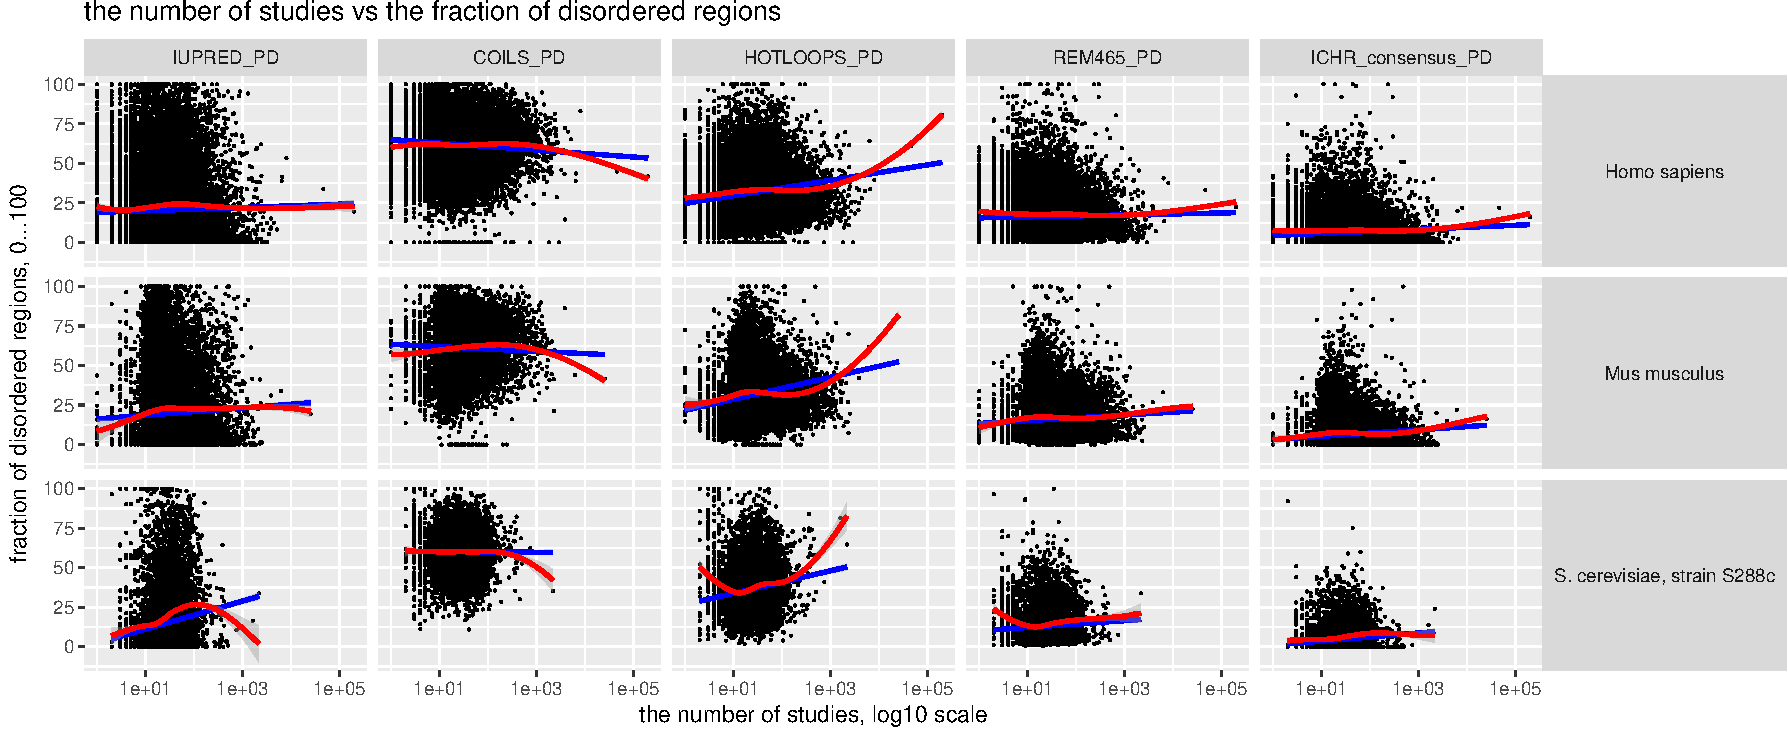
\includegraphics{final_report_files/figure-latex/disord_domain_vs_publications-1.pdf}

The second plot is a quantile-quantile plot which shows that the
distribution of the fraction of disordered domains is far from normal.
Square root or logarithmic transformations do not change that.

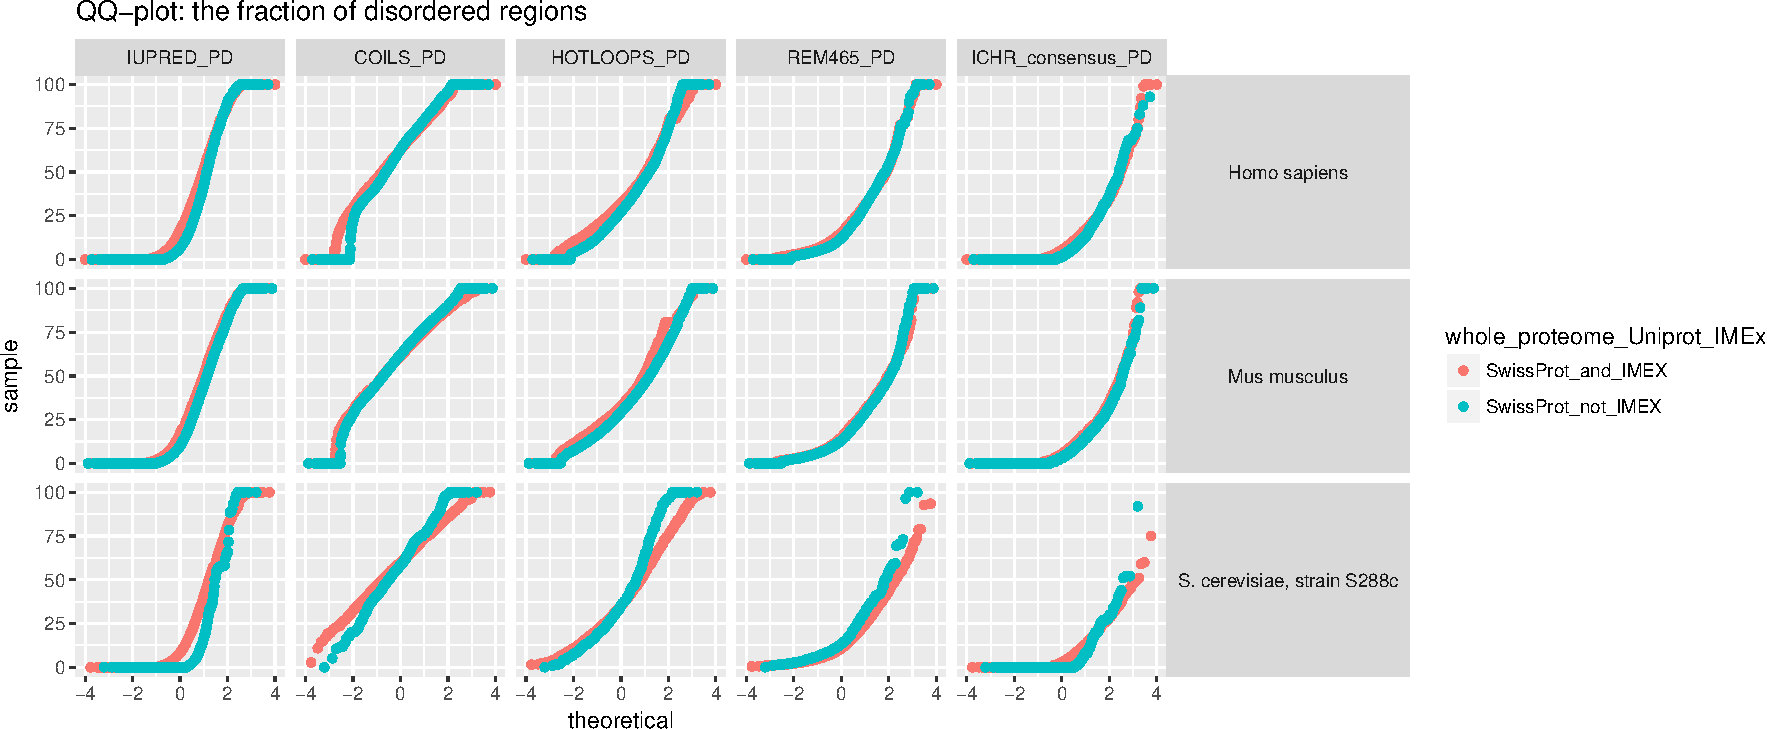
\includegraphics{final_report_files/figure-latex/disord_domain_vs_publications_qqplot-1.pdf}

From these graphs, we can conclude that the fraction of disordered
domains can vary depend on the number of studies and disordered region
prediction algorithm (which may reflect the bias of disordered region
prediction algorithms.

\subsubsection{Proteins with a low fraction of disordered domains tend
to have fewer
interactions}\label{proteins-with-a-low-fraction-of-disordered-domains-tend-to-have-fewer-interactions}

If disordered regions are often needed for molecular interactions we
would expect that proteins with a higher fraction of disordered regions
will tend to have more interacting partners (irrespective of the study
bias).

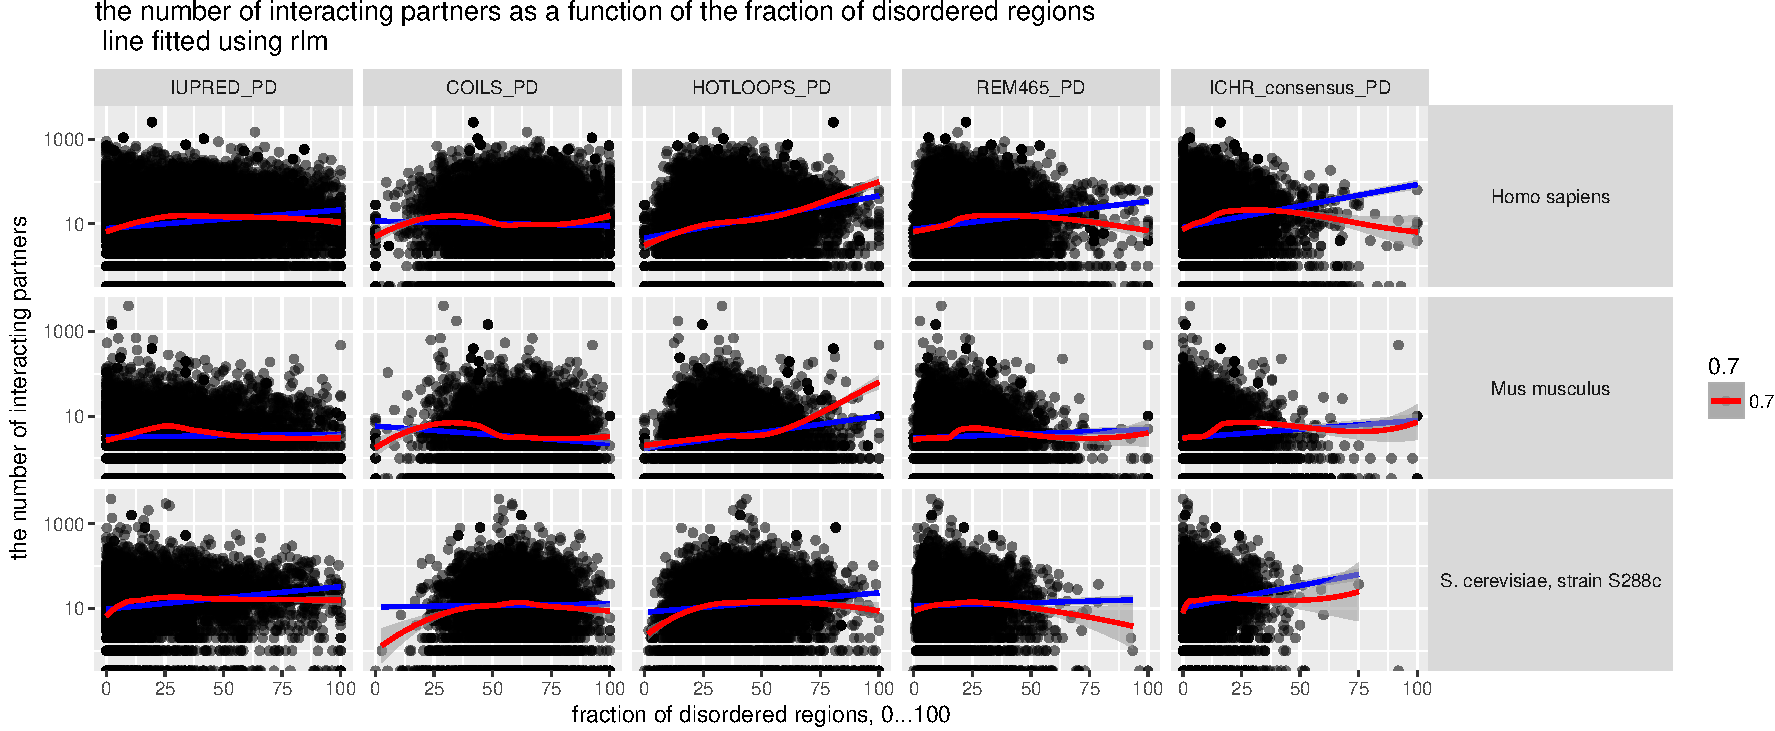
\includegraphics{final_report_files/figure-latex/disord_domain_vs_n_interactions-1.pdf}

As you can see from the loess-fitted curve (red, loess stands for local
polynomial regression), the proteins with a low fraction of disordered
domains tend to have fewer interactions while further increasing the
fraction of disordered regions doesn't change the trend. The more
general trend is shown in blue - robust linear regression. Whether these
trends are the result of chance or study bias is yet to be tested.

\subsubsection{The longer yeast protein is the more interactions it has
(doesn't hold true for
mouse)}\label{the-longer-yeast-protein-is-the-more-interactions-it-has-doesnt-hold-true-for-mouse}

In theory, the length of the protein can influence the number of
interaction partners of the protein: the longer the protein the more
functional and structural domains it has and the more molecular
interactions that function will require.

\includegraphics{final_report_files/figure-latex/protein_mass_vs_n_interactions-1.pdf}

The analysis shows that the number of interacting partners correlates
with the protein length in yeast, but not in human or mouse.

\subsubsection{The length of the disordered regions and the number of
interactions}\label{the-length-of-the-disordered-regions-and-the-number-of-interactions}

The sum length of disordered regions per protein can be a better
predictor of the number of interacting partners because it captures both
the presence of disordered regions and the fact that longer proteins
have more functional domains.

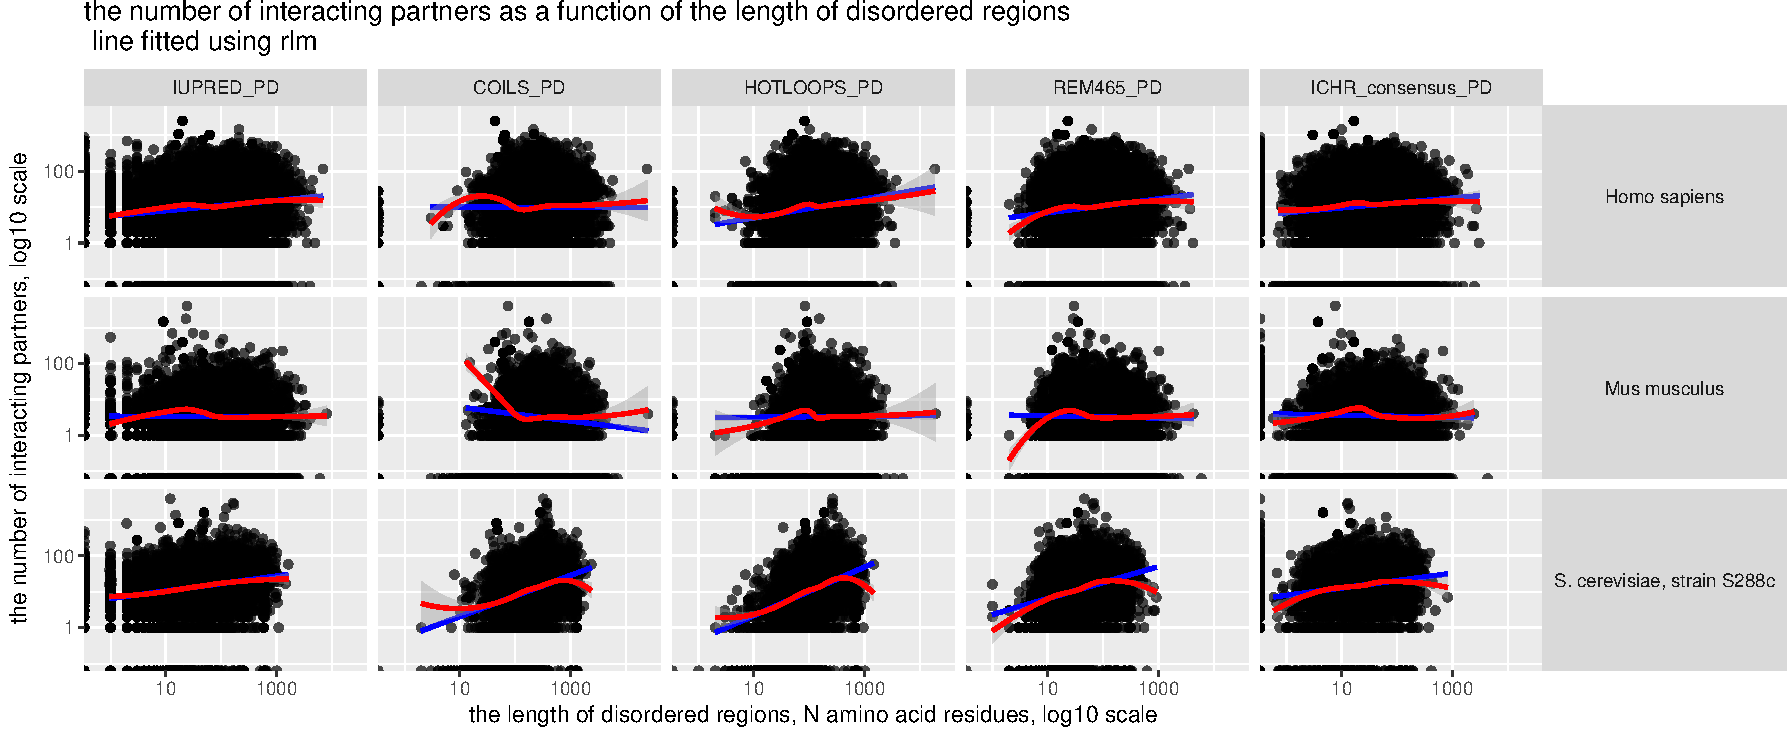
\includegraphics{final_report_files/figure-latex/protein_mass*disord_domain_vs_n_interactions-1.pdf}

\subsection{10. The number of protein domains (InterPro) and the number
of
interactions}\label{the-number-of-protein-domains-interpro-and-the-number-of-interactions}

\includegraphics{final_report_files/figure-latex/N_domain_vs_n_publications-1.pdf}

\includegraphics{final_report_files/figure-latex/N_domain_vs_n_interactions-1.pdf}

coming soon

\section{Supplementary figures}\label{supplementary-figures}

Supplementary figure 1

\begin{figure}[htbp]
\centering
\includegraphics{final_report_files/figure-latex/Supplementary1_IMEx_vs_Uniprot_venndiagram_all_Uniprot-1.pdf}
\caption{Supplementary figure 1. The overlap between proteins with known
interactions (interactome) and all proteins included in UniprotKB
(proteome)}
\end{figure}

\begin{figure}[htbp]
\centering
\includegraphics{final_report_files/figure-latex/Supplementary2_BioGRID_vs_IMEx_vs_Uniprot_N_Uniprot_Species-1.pdf}
\caption{Supplementary figure 2. The number of interacting proteins from
given species or the other species in BioGRID}
\end{figure}

\begin{figure}[htbp]
\centering
\includegraphics{final_report_files/figure-latex/Supplementary3_protein_mass_distribution_qqplot-1.pdf}
\caption{Supplementary figure 3. Proteomes have much more long proteins
than normal distribution would predict (proteins, dots, are above the
line in qqplot). The distribution of logarhithm base 10 of protein mass
is approximately normal}
\end{figure}

\begin{figure}[htbp]
\centering
\includegraphics{final_report_files/figure-latex/Supplementary4_protein_mass_distribution_monte_carlo-1.pdf}
\caption{Supplementary figure 4. Monte-Carlo sampling of can indentify
the difference in protein mass between proteins present and missing from
IntAct}
\end{figure}

\begin{figure}[htbp]
\centering
\includegraphics{final_report_files/figure-latex/Supplementary4_protein_mass_distribution_permutations-1.pdf}
\caption{Supplementary figure 4. Permutation of labels (does have
interactions / doesn't have interactions) the difference in protein mass
between proteins present and missing from IntAct}
\end{figure}


\end{document}
